\toptitle{[ELEC-H-201] Électricité et électronique}{TP1b}
\TPtitle{Électricité et électronique\vspace*{2mm}}{TP1b:\vspace*{2mm} 
Circuits réactifs en régime sinusoïdal permanent}

\frontpage{consignes1b.tex}
\vspace{5cm}
\newpage

\section{Exercice 1}
Sur le circuit suivant, excité par une tension sinusoïdale, on a mesuré l’amplitude des tensions $v_S(t)$ et $v_R(t)$. Cela donne respectivement $500mV$ et $300mV$. 
\begin{center}
\begin{circuitikz} \draw
(0,0)	to[sinusoidal voltage source, v=$v_S(t)$, i_>=$i(t)$]		(0,3)
		to[R, l_=$R$, v^<=$v_R(t)$]					(3,3)
		to[C, l_=$C$, v^<=$v_C(t)$]					(3,0)--(0,0)
;
\end{circuitikz}
\end{center}
\Question{0}
{%Q
On demande d’en déduire l’amplitude de la tension $v_C(t)$.
}
{
On pourrait penser que l'amplitude de $v_C(t)$ est la différence des deux : $\widehat{V}_C=\widehat{V}_S-\widehat{V}_R=500mV-300mV=200mV$.\\
Ce n’est pas le cas ! En effet les deux sinusoïdes n’ont pas la même phase : comme on le verra à l’exercice suivant, la tension $v_C(t)$ est en retard de 90° sur la tension $v_R(t)$, qui est elle en phase avec le courant. Ceci nous permet d’emblée poser un point important :  on ne peut pas sommer les amplitudes des tensions ou des courants ! En revanche, on peut sommer les équations temporelles ou les phaseurs qui leur correspond.\\
On s’aperçoit que l’on obtient un triangle rectangle, et que donc $\widehat{V}_C=\sqrt{\widehat{V}_S^2-\widehat{V}_R^2}=400mv$.\\
Par ailleurs la phase de $v_S(t)$ est donnée par $\Phi=-atan(\frac{\widehat{V}_C}{\widehat{V}_R})$.
}
\Question{0}
{
Repartez du même circuit. On donne cette fois le courant parcourant la boucle: $i(t)=10^{-3}\times cos(2,5 \times 10^4t)\ [A]$. Vous savez également que $R=300\Omega$ et que $C=100nF$. En vous basant sur les lois des dipôles, trouvez la variation temporelle de Vs. On demande une réponse de la forme $v_S(t)=A\times  cos(\omega t+\Phi)\ [V]$.
}
{
\textbf{Méthode 1 : résolution dans le domaine temporel}\\
Par définition :\\
$$v_R(t)=Ri(t)=0,3\times \cos(2,5\times 10^4 t)\ [V]$$
$$v_C(t)=\frac{1}{C} \int{i(t)dt}=\frac{10^{-3}}{2,5\times 10^4 C}sin(2,5 \times 10^4 t)=0,4\times sin(2,5 \times 10^4 t)\ [V]$$\\
On a : $$v_S (t)=0,3\times cos(2,5 \times 10^4 t)+0,4\ \times  sin(2,5 \times 10^4 t)$$
D’après les formules de Simpson : 
$$cos(a)\times cos(b)-sin(a)\times sin(b)=cos(a+b)$$
$$\Rightarrow A\times (cos(\omega t)\times cos(\Phi))-sin(\omega t)\times sin(\Phi))=A\times cos(\omega t+\Phi)$$
On en tire $A\times cos(\Phi)=0,3V$ et $A\times sin(\Phi)=-0,4V$, soit encore $$A=\widehat{V}_S=\sqrt{(0,3V)^2+(0,4V)^2}=0,5V$$
$$\Phi_{V_S}=-atan(\frac{0,4V}{0,3V})=-53^o=-0,93rad$$
$$\Rightarrow v_S(t)=\widehat{V}_S\times cos(2,5 \times 10^4 t+\Phi_{V_S})$$

\textbf{Méthode 2 : résolution dans le domaine fréquentiel (phaseurs)}\\
$$\underline{V}_S=\underline{V}_R+\underline{V}_C=Z_R\underline{I}+Z_C\underline{I}=(R+\frac{1}{j\omega C})\underline{I}=\frac{1+j\omega RC}{j\omega C}\times \underline{I}$$
$$=\frac{|1+j\omega RC|}{|j\omega C|}e^{j(atan(\frac{\omega RC}{1})-atan(\frac{\omega C}{0}))} |\underline{I}|e^{j\Phi_I}$$
$$\Rightarrow \widehat{V}_S=|\underline{V}_S|=\frac{|1+j\omega RC|}{|j\omega C|}|I|=\frac{\sqrt{1+(\omega RC)^2}}{\omega C}|I|=\frac{\sqrt{1+(0,75)^2}}{2,5\times 10^{-3}}\times 10^{-3}=0,5V$$
$$\Rightarrow \Phi_{V_S}=Arg(\underline{V}_S)=atan(\frac{\omega RC}{1})-atan(\frac{\omega C}{0})+\Phi_I=atan(0,75)-90°+0$$
$$=37°-90°=-53°=-0,93rad$$
Cela donne donc bien les mêmes valeurs que celles obtenues dans le domaine temporel:
$$\Rightarrow v_S(t)=\widehat{V}_S\times cos(2,5 \times 10^4 t+\Phi_{V_S})$$
}
\Question{0}
{
Comparez vos réponses des points 1 et 2. Qu’en concluez vous ?
}
{On constate que les réponses sont identiques. En revanche le raisonnement tenu pour les phaseurs est manifestement plus simple. Ces derniers permettent par ailleurs une représentation simple et condensée ne faisant plus apparaître le temps.\\
Et c’est normal : lorsque l’on excite un circuit linéaire par une sinusoïde, toutes les tensions et courants seront aussi des sinusoïdes d’amplitude et de phase diverses, mais de même fréquence. De ce fait il n’est pas la peine d’alourdir les calculs : l’amplitude et la phase suffisent pour décrire entièrement un signal.}

\section{Exercice 2}

Voici 3 dipôles:
\begin{center}
\begin{circuitikz} \draw
(0,0)	to[C, v<=$V_C$, l=$1\mu F$, i=$i$]			(3,0)
(5,0)	to[R, v<=$V_R$, l=$300\Omega$, i=$i$]		(8,0)
(10,0)	to[L, v<=$V_L$, l=$200\mu H$, i=$i$]		(13,0)
;
\end{circuitikz}
\end{center}
\Question{0}
{On fait passer un courant de $20mA$ d’amplitude et d’une fréquence de $1591Hz$ dans ces dipôles. Pour chacun d’entre eux, calculez le phaseur de la tension à ses bornes, tracez ce dernier dans le plan complexe et déduisez-en l’impédance du dipôle.
}
{
Le courant est de la forme $i(t)=\widehat{I} cos(\omega t)$  avec $\omega=2\pi f$, et son phaseur est $$\underline{I}=|\underline{I}|e^{jArg(\underline{I})}=\widehat{I}e^{j\Phi_I}=20\times 10^{-3}e^{j0°}=20\times 10^{-3}\ [A]$$

Prenons, $i(t)=\widehat{I}cos(\omega t+\Phi_I)=20\times 10^{-3}cos(2\pi \times 1591\times t)$. On prend le courant comme référence de phase: $\Phi_I=0$.\\
Par la loi du \textbf{condensateur} :
$$v_C(t)=\frac{1}{C} \int{i(t)dt}=\frac{1}{\omega C}\widehat{I}\times sin(\omega t)=\frac{1}{\omega C}\widehat{I}\times cos (\omega t-\frac{\pi}{2})$$
Le phaseur associé est
$$\underline{V}_C=\frac{1}{\omega C}\widehat{I}e^{-j\frac{\pi}{2}}=-j\frac{1}{\omega C}\widehat{I}=\frac{1}{j\omega C}\widehat{I}=\frac{1}{j\times 2\pi\times 1591\times 10^{-6}}20\times 10^{-3}$$
$$=-j100\times 20\times 10^{-3}=-j2\ [V]$$
L’impédance de la capacité est donc
$$Z_C=\frac{\underline{V}_C}{\underline{I}}=\frac{1}{j\omega C}=\frac{1}{j\times 2\pi \times 1591 \times 10^{-6}}=-j\frac{1}{10^4 \times 10^{-6}}=-j100\Omega$$
\vspace{-5mm}
\begin{center}
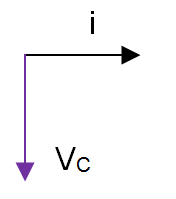
\includegraphics[scale=0.5]{TP1_EXO1b_Q2_1_C.PNG}
\end{center}

Par loi de la \textbf{résistance} :
$$v_R(t)=R i(t)=R\widehat{I} cos(\omega t)$$
Le phaseur associé est $\underline{V}_R=R\underline{I}=300\times 20\times 10^{-3}=6\ [V]$.\\
L'impédance d'une résistance est donc $Z_R=\frac{\underline{V}_R}{\underline{I}}=300\Omega$
\begin{center}
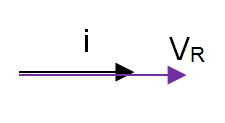
\includegraphics[scale=0.5]{TP1_EXO1b_Q2_1_R.PNG}
\end{center}

Par la loi de l’\textbf{inductance} :
$$v_L(t)=L\frac{di(t)}{dt}=-\omega L sin(\omega t)=\omega L\widehat{I} cos(\omega t+\frac{\pi}{2})$$
Le phaseur associé est 
$$\underline{V}_L=\omega L \widehat{I}e^{j \frac{\pi}{2}}=j\omega L\underline{I}=j\times 2\pi \times 1591 \times 200 \times 10^{-6} \times 20 \times 10^{-3}= j4\times 10^{-2}\ [V]$$

L'impédance de l'inductance est donc $Z_L=\j\omega L=j\times 10^4\times 200 \times 10^{-6}=j2 \Omega$.
\begin{center}
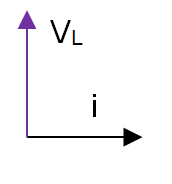
\includegraphics[scale=0.5]{TP1_EXO1b_Q2_1_L.PNG}
\end{center}

%Le phaseur associé est $\underline{V}_L=\omega L \frac{I}{sqrt{2}}e^{j \pi/2} I/√2  e^(jπ/2)=j\omega L\underline{I}=j 20\sqrt{2}mV.\\
% L’impédance de l’inductance est donc $Z_L=j\omegaL= j\sqrt{2} \Omega$.
}
\Question{0}
{
Par quoi peut-on remplacer un condensateur excité par un signal à très basse fréquence ? Et à très haute fréquence ?
}
{
On sait que $Z_C=\frac{1}{j\omega C}$.\\

Pour une fréquence très basse, $\omega \rightarrow 0 \Rightarrow Z_C \rightarrow \infty$.\\
On peut donc la remplacer par un circuit ouvert (analogie avec la loi long terme : le courant continu est nul dans une capacité).\\

Pour une fréquence très élevée, $\omega \rightarrow \infty \Rightarrow Z_C \rightarrow 0$.\\
On peut donc la remplacer par un court-circuit.
}

\Question{0}
{
Par quoi peut-on remplacer une inductance excitée par un signal à très basse fréquence ? Et à très haute fréquence ?
}
{
On sait que $Z_L=j\omega L$.\\

Pour une fréquence très basse, $\omega \rightarrow 0 \Rightarrow Z_L \rightarrow 0$.\\
On peut donc la remplacer par un court-circuit (analogie avec la loi long terme : la tension continue aux bornes d’une inductance est nulle).\\

Pour une fréquence très élevée :$\omega \rightarrow \infty \Rightarrow Z_L \rightarrow \infty$,\\
On peut donc la remplacer par un circuit ouvert.
}



%%%%%%%%%%%%%%%%%%%%%%%%%%
%       ANCIEN EXO
%%%%%%%%%%%%%%%%%%%%%%%%%%
% La tension $e(t)=V_m \cos(\omega t+\alpha)$ est appliquée à l'instant $t=T_0=0$ au circuit $RL$.
% \begin{center}
% \begin{circuitikz} \draw
% (0,0)	to[sinusoidal voltage source, v=$e(t)$, i=$i$]		(0,4)
% 		to[closing switch, l=$T_0$]		(3,4)
% 		to[R, l=$R$]					(3,2)
% 		to[L, l=$L$]					(3,0)--(0,0)
% ;
% \end{circuitikz}
% \end{center}

% \Question{0}
% {%Q
% \textit{Discuter la valeur de $\alpha$ pour que:
% \begin{enumerate}
% \item le régime permanent s'établisse immédiatement
% \item la valeur instantanée du courant soit maximale
% \end{enumerate}}
% }
% {%C
% La solution générale est (cfr cours):
% $$i(t)=i'(t)+i''(t)=I_m \cos(\omega t + \alpha -\theta) - I_m \cos(\alpha -\theta) e^{-t/\tau}$$
% Où $i'(t)$ est le terme de régime et $i''(t)$, le terme transitoire.
% \begin{multicols*}{3}
% $$I_m=\frac{V_m}{\sqrt{R^2}+\omega^2+L^2}$$
% \newpage
% $$tan(\theta)=\frac{\omega L}{R}$$
% \newpage
% $$\tau=\frac{L}{R}$$
% \end{multicols*}
% Le transitoire est nul si $\cos(\alpha -\theta)=0 \Leftrightarrow \alpha -\theta=\pm \pi/2$.\\
% Cela correspond à un enclenchement du circuit ($t=0$) au moment où le terme de régime passe par zéro. Dans ce cas, le régime permanent s'établit immédiatement.\\

% Le terme transitoire sera maximum lorsque le circuit est enclenché au moment où le terme de régime passe par son maximum positif ou négatif ($\pm I_m$).
% $$\alpha - \theta =0 \ ou \ \pi \Leftrightarrow i(t)=\pm I_m (\cos(\omega t) - e^{-\frac{R}{L}t})$$
% Si $\omega L >> R$, le terme transitoire garde une valeur appréciable pendant plusieurs période.\\
% Dans ce cas, le courant total atteint sa valeur maximale $i_{max}$ environ à 1/2 période après le branchement, lorsque le terme de régime s'approche de sa valeur maximale, mais a le même signe que le terme transitoire:
% $$i_{max}=i(T/2)\simeq I_m (1+e^{-\frac{R}{L}\frac{T}{2}})=I_m (1+e^{-\pi \frac{R}{\omega L}}) \simeq 2I_m \ (si \frac{R}{\omega L} est petit)$$
% \begin{center}
% \includegraphics[scale=0.25]{TP3-Exo1.png}
% \end{center}
% }

%Corrigé ancien Exo 2
%$(R_1+R_2+j\omega L+\frac{1}{j\omega C_1})\underline{I}_1-(R_2+\frac{1}{j\omega C_1}\underline{I}_2=\underline{E}_1$\\
%$-(R_2+\frac{1}{j\omega C_1})\underline{I}_1+(R_2+R_3+\frac{1}{j\omega C_1}+\frac{1}{j\omega C_2})\underline{I}_2=-\underline{E}_2$\\
%
%$\Leftrightarrow (9+j3)\underline{I}_1-(4-j3)\underline{I}_2=50e^{j20^o}$\\
%$\hspace{9mm} -(4-j3)+(8-j8)\underline{I}_2=-60e^{-j30^o}$

\section{Exercice 3}
Soit le circuit suivant où $v_S(t)=\widehat{V}_S\times cos(\omega t+ \Phi_{V_S})$, $\widehat{V}_S=2V$, $\omega=10^6rad/s$, $\Phi_{V_S}=20°$, $R_1=100\Omega$, $R_2=200\Omega$ et $R_3=200\Omega$.
\begin{center}
\begin{circuitikz} \draw
(0,0)	to[sinusoidal voltage source, i_>=$i(t)$, v=$v_S(t)$]		(0,2)
		to[R, l=$R_1$]					(2,2)--(4,2)
(2,2)
		to[R, l_=$R_2$]		(2,0)
(4,2)	to[R, l_=$R_3$, v^<=$v_2(t)$]					(4,0)--(0,0)
;
\end{circuitikz}
\end{center}

\Question{0}
{ 
Que vaut la tension $v_2(t)$ de ce circuit?
}
{ 
En mettant $R_2$ et $R_3$ en parallèle, on obtient la résistance équivalente
$$R_{23}=R_2//R_3=\frac{R_2R_3}{R_2+R_3}=100\Omega$$
La tension $v_2(t)$ est alors celle au borne de $R_{23}$.\\
Par le diviseur résistif:
$$v_2(t)=\frac{R_{23}}{R_{23}+R_1}v_S(t)=\frac{100}{200}=0,5v_S(t)=\widehat{V}_2\times cos(\omega t+ \Phi_{V_2})$$
Avec $\widehat{V}_2=1V$, $\omega=10^6rad/s$, et $\Phi_{V_2}=20°$.
}

Soit le circuit suivant où $v_S(t)=\widehat{V}_S\times cos(\omega t+ \Phi_{V_S})$, $\widehat{V}_S=2V$, $\omega=10^6rad/s$, $\Phi_{V_S}=20°$, $R_1=100\Omega$, $R_2=137\Omega$ et $L=100\mu F$.
\begin{center}
\begin{circuitikz} \draw
(0,0)	to[sinusoidal voltage source, i_>=$i(t)$, v=$v_S(t)$]		(0,2)
		to[R, l=$R_1$]					(2,2)--(4,2)
(2,2)
		to[R, l_=$R_2$]		(2,0)
(4,2)	to[L, l_=$L$, v^<=$v_2(t)$]					(4,0)--(0,0)
;
\end{circuitikz}
\end{center}

\Question{0}
{ 
Que vaut la tension $v_2(t)$ de ce circuit?
}
{ 
Essayons de retrouver une forme semblable au diviseur résistif, mais dans le domaine fréquentiel (avec les phaseurs).\\
En mettant $R_2$ et $L$ en parallèle, on obtient l'impédance équivalente: $$Z_{eq}=\frac{j\omega LR_2}{R_2+j\omega L}$$
La tension $v_2(t)$ est alors celle au borne de $Z_{eq}$.\\
Par le diviseur impédant:
$$\underline{V}_2=\frac{Z_{eq}}{Z_{eq}+R_1}\underline{V}_S=\frac{\frac{j\omega LR_2}{R_2+j\omega L}}{R_1+\frac{j\omega LR_2}{R_2+j\omega L}}\underline{V}_S=\frac{j\omega LR_2}{R_1R_2+j\omega L(R_1+R_2)}\underline{V}_S$$
$$=\frac{j1,37\times 10^4}{1,37\times 10^4+j2,37\times 10^4}\underline{V}_S=\frac{1,37}{\sqrt{1,37^2+2,37^2}}e^{j(\frac{\pi}{2}-atan(\frac{2,37}{1,37}))}\underline{V}_S=\frac{1}{2}e^{j30^o}\underline{V}_S$$.\\

Et, en écrivant le phaseur de la tension d'entrée: $\underline{V}_S=2\times e^{j20^o}$, on a:
$$\underline{V}_2=2V\times \frac{1}{2}e^{j(20^o+30^o)}=e^{j50^o}$$

Enfin, la variation temporelle est
$$v_2(t)=Re(\underline{V}_2e^{j\omega t})=Re(e^{j(\omega t+50^o)}=cos(\omega t+50^o)=\widehat{V}_2\times cos(\omega t+ \Phi_{V_2})$$
Avec $\widehat{V}_2=1V$, $\omega=10^6rad/s$, et $\Phi_{V_2}=50°$.\\

Ce calcul impliquant des phaseurs parait long, mais résoudre le circuit à partir des équations temporelles aurait été encore nettement plus compliqué.

%La loi de la résistance $R_1$ est $\underline{V}_S-V_2=Z_{R_1}\underline{I}$.\\
%Par la loi des nœuds : $$\underline{I}=\frac{\underline{V}_2}{Z_{R2} +Z_L} 
% En mettant ensemble : ▁(V_2 )=(Z_R2 Z_L)/(Z_R2 Z_L+Z_R1 ) ▁(V_in ). Cette formule est très importante car elle montre que pour autant que l’on utilise les phaseurs et les impédances, on peut appliquer presque tels quels les principes vus pour la résistance. Cette extension du diviseur résistif se nomme diviseur d’impédance.
% De cette formule, on tire 
% ▁(V_2 )=(jωLR_2)/(jωL(R_1+R_2)+R_1 R_2 ) ▁(V_in )=(j 1.37 〖10〗^4)/(j 2.37 〖10〗^4+1.37 〖10〗^4 ) ▁(V_in )=1.37/√(〖2.37〗^2+〖1.37〗^2 ) e^(j π/2-j atan⁡(2.37/1.37) ) ▁(V_in )=1/2 e^(j30°)  ▁(V_in )
% Et, en écrivant le phaseur de la tension d’entrée : ▁(V_in )=2V e^(j20°), on a
% ▁(V_2 )=2V*1/2  e^(j20°+j30°)=1V e^(j50°)
% Enfin la variation temporelle est V_2 (t)=√2 Re (▁(V_2 )  e^jωt )=√2 Re (1V e^j(ωt+50°)  )=√2 V cos⁡〖(ωt+50°)〗.
% Ce calcul impliquant des phaseurs parait long, mais résoudre le circuit à partir des équations temporelles aurait été encore nettement plus compliqué.
}


\section{Exercice 4}
Pour le circuit suivant
\begin{center}
\begin{circuitikz} \draw
(0,0)	to[sinusoidal voltage source, v=$v_S(t)$, i_>=$i(t)$]		(0,4)
		to[R, l=$R_1$]					(2,4)--(4,4)
(0,0)--(4,0)
		to[capacitor, l=$C$, v>=$v_C(t)$]		(4,4)
(2,4)	to[R, l=$R$]					(2,2)
		to[L, l=$L$]					(2,0)
;
\end{circuitikz}
\end{center}
Où $v_S(t)=\widehat{V}_S\times cos(\omega t+ \Phi_{V_S})$, $\widehat{V}_S=1V$, $\omega=4rad/s$, $\Phi_{V_S}=45°$, $R_1=4\Omega$, $R=1\Omega$, $L=1H$ et $C=\frac{1}{4}F$

\Question{0}
{%Q
\textit{Déterminer la tension aux bornes de la capacité $V_C(t)$.}
}
{%C
On place d'abord les flèches de tensions et courants:
\begin{center}
\begin{circuitikz} \draw
(0,0)	to[sinusoidal voltage source, v=$V_S(t)$, i_>=$i(t)$]		(0,4)
		to[R, l=$R_1$]					(2,4)--(4,4)
(0,0)--(4,0)
		to[capacitor, l=$C$, v>=$V_C(t)$, i<^=$i_C(t)$]		(4,4)
(2,4)	to[R, l=$R_2$, i_=$i_L(t)$]					(2,2)
		to[L, l=$L$]					(2,0)
;
\end{circuitikz}
\end{center}
Il s'agit d'une circuit avec source sinusoïdale en régime permanent, la résolution  se fera donc dans le domaine fréquentiel, avec l'aide des phaseurs.\\
Plusieurs méthodes de résolution sont possibles.\\
\textbf{Méthode 1 : }\\
$$\underline{V}_S=R_1\underline{I}+\underline{V}_C=R_1(\underline{I}_L+\underline{I}_C)+\underline{V}_C$$
$$\underline{V}_C=(R+j\omega L)\underline{I}_L \Rightarrow \underline{I}_L=\frac{\underline{V}_C}{R_2+j\omega L}$$
$$\underline{V}_C=\frac{\underline{I}_C}{j\omega C} \Rightarrow \underline{I}_C=j\omega C \underline{V}_C$$
Avec ce système d'équations, on trouve donc:
$$\underline{V}_S=\frac{R_1}{R_2+j\omega L}\underline{V}_C+j\omega R_1 C \underline{V}_C+\underline{V}_C=\frac{R_1+R_2-\omega^2R_1LC+j\omega(L+R_1R_2C)}{R_2+j\omega L}\underline{V}_C$$
On a donc:
$$\underline{V}_C=\frac{R_2+j\omega L}{R_1+R_2-\omega^2R_1LC+j\omega(L+R_1R_2C)}\underline{V}_S$$
Comme $v_S(t)=\widehat{V}_S\times cos(\omega t+ \Phi_{V_S})$, avec les valeurs données dans l'énoncé, son phaseur (phaseurs en sinus, sinon, déphaser de $90^o$) est $\underline{V}_S=e^{j45^o}$. On remplace dans l'expression du phaseur de $v_C(t)$:
$$\underline{V}_C=e^{j45^o}\frac{1+j4}{-11+j8}=e^{j45^o}\frac{4,12e^{j75,96^o}}{13,6e^{j143,97^o}}=0,303e^{-j23^o}$$
Et donc, lorsqu'on repasse dans le domaine temporel:
$$v_C(t)=\widehat{V}_C\times cos(\omega t+ \Phi_{V_C})$$
Avec $\widehat{V}_C=0,303V$, $\omega=4rad/s$, et $\Phi_{V_C}=-23°$.\\

\textbf{Méthode 2 : }\\
Une autre méthode possible est l'utilisation du diviseur impédant.
On remplace $R_2$, $L$ et $C$ par une impédance équivalente:
$$Z_{eq}=(Z_R+Z_L)//Z_C=\frac{(R_2+j\omega L)\frac{1}{j\omega C}}{R_2+j\omega L+\frac{1}{j\omega C}}=\frac{R_2+j\omega L}{1-\omega^2LC+j\omega R_2C}$$
Ensuite, par le diviseur impédant:
$$\underline{V}_C=\frac{Z_{eq}}{Z_{eq}+R_1}\underline{V}_S=\frac{\frac{R_2+j\omega L}{1-\omega^2LC+j\omega R_2C}}{R_1+\frac{R_2+j\omega L}{1-\omega^2LC+j\omega R_2C}}\underline{V}_S=\frac{R_2+j\omega L}{R_1+R_2-\omega^2R_1LC+j\omega(L+R_1R_2C)}\underline{V}_S$$
On retombe donc bien sur la même équation que celle obtenue par la première méthode!
}

%%%%%%%%%%%%%%%%%%%%%%%%%%
%       ANCIEN EXO
%%%%%%%%%%%%%%%%%%%%%%%%%%
% \section{Exercice 3}
% Le circuit suivant se trouve en régime à l'instant $t=T_0=0$ de fermeture de l'interrupteur. 
% \begin{center}
% \begin{circuitikz} \draw
% (0,0)	to[sinusoidal voltage source, l=$e(t)$]		(0,2)
% 		to[R, l=$R_1$]								(2,2)
% 		to[closing switch, l=$T_0$]					(4,2)
% 		to[R, l=$R_2$]								(4,0)--(0,0)
% (2,2)	to[C, l=$C$]								(2,0)
% ;
% \end{circuitikz}
% \end{center}
% \Question{0}
% {%Q
% \textit{Déterminer les courants pour toute valeur de $t$, avec $e(t)=E_0 \cos(\omega t)$.}
% }
% {%C
% \begin{center}
% \begin{circuitikz} \draw
% (0,0)	to[sinusoidal voltage source, l=$e(t)$]		(0,2)
% 		to[R, l=$R_1$, i=$i_0$]								(2,2)
% 		to[closing switch, l=$T_0$]					(4,2)
% 		to[R, l=$R_2$, i=$i_2$]								(4,0)--(0,0)
% (2,2)	to[C, l=$C$, i=$i_1$]								(2,0)
% ;
% \end{circuitikz}
% \end{center}

% \begin{itemize}
% \item \textbf{Pour $t<0$ (état de régime)}\\
% $\underline{I}_0=\frac{E_0}{R_1+\frac{1}{j\omega C}}=\frac{j\omega CE_0}{1+j\omega CR_1}$\\
% $i_0(t)=\frac{\omega CE_0}{\sqrt{1+\omega^2 C^2 R_1^2}}\cos(\omega t+\phi)$ avec $tan(\phi)=\frac{1}{\omega CR_1}$\\
% $i_1(t)=i_0(t)$ et $i_2(t)=0$\\
% $\underline{V}_C=\frac{\underline{I}_0}{j\omega C}=\frac{E_0}{1+j\omega CR_1}$\\
% $\Rightarrow v_C(t)=\frac{E_0}{\sqrt{1+\omega^2 C^2 R_1^2}}\cos(\omega t-\alpha)$ et $tan(\alpha)=\omega CR_1$
% \item \textbf{Pour $t>0$}\\
% $E_0 \cos(\omega t)=R_1(i_1+i_2)+R_2i_2$ \hspace{1cm}$(1)$\\
% $v_C(0)+\frac{1}{C}\int_0^t i_1dt=R_2i_2 \Rightarrow i_1=CR_2\frac{di_2}{dt}$\hspace{1cm}$(2)$\\
% $(1)$ et $(2)$ $\Rightarrow E_0 \cos(\omega t)=(R_1+R_2)i_2+CR_1R_2\frac{di_2}{dt}$\\
% $\Rightarrow i_2(t)=Ae^{-t\frac{R_1+R_2}{CR_1R_2}}+sol.\ partic.$\\

% Pour chercher la solution particulière en $t>0$, $i_{2_p}(t)$, on va utiliser la méthode des phaseurs:\\
% $\frac{1}{j\omega C}\underline{I}_1=R_2\underline{I}_2$\\
% $\underline{E}_0=R_1(\underline{I}_1+\underline{I}_2)+R_2\underline{I}_2$\\

% $\Rightarrow \underline{I}_2=\frac{E_0}{R_1+R_2+j\omega CR_1R_2}$\\
% $\underline{I}_1=\frac{j\omega CR_2E_0}{R_1+R_2+j \omega CR_1R_2}$\\

% La solution particulière est donc:\\
% $$i_{2_p}(t)=K \cos(\omega t-\beta)$$
% où $K=\frac{E_0}{\sqrt{(R_1+R_2)^2+(\omega CR_1R_2)^2}}$, $tan(\beta)=\omega \tau$ et $\tau=\frac{R_1R_2C}{R_1+R_2}$\\

% La solution générale pour $t>0$ est alors:\\
% $i_2(t)=Ae^{-t/\tau}+K \cos(\omega t-\beta)$\\
% et il faut identifier $A$ à partir de la condition initiale.\\

% \item \textbf{Condition initiale ($t=0^+$)}\\
% $i_2(0^+)=\frac{v_C(0^+)}{R_2}=\frac{v_C(0^-)}{R_2}=\frac{E_0 \cos(\alpha)}{R_2\sqrt{1+\omega^2 C^2 R_1^2}}$\\
% $A=\frac{E_0 \cos(\alpha)}{R_2\sqrt{1+\omega^2 C^2 R_1^2}}-K\cos(\beta)$\\

% On a $i_2(t)$ pour $t>0$ (ouf!):\\
% $i_2(t)=Ae^{-t/\tau}+K \cos(\omega t-\beta)$\\
% $i_2(t)=\frac{E_0 \cos(\alpha)}{R_2\sqrt{1+\omega^2 C^2 R_1^2}}-K\cos(\beta)e^{-t\frac{R_1+R_2}{R_1R_2C}}+\frac{E_0}{\sqrt{(R_1+R_2)^2+(\omega CR_1R_2)^2}}\cos(\omega t-\beta)$

% \item \textbf{Pour les autres courants en $t>0$}\\
% $i_1(t)=CR_2\frac{di_2}{dt}=-\frac{CR_2}{\tau}Ae^{-t/\tau}-KCR_2\omega \sin(\omega t-\beta)$\\
% $i_0(t)=i_1(t)+i_2(t)$
% \end{itemize}
% }


\section{Exercice 5}
Le signal $v_e(t)$ à mesurer est connecté à un oscilloscope au moyen d'une sonde externe. La sonde est constituée d'une résistance $R_S$ et d'une capacité $C_S$ (réglable) en parallèle.\\
L'impédance d'entrée de l'oscilloscope est modélisée par la mise en parallèle de $R_{in}=1M\Omega$ et $C_{in}=20pF$.\\
 
\begin{center}
\begin{circuitikz} \draw
node[ocirc] (A) at (0,2) {}
node[ocirc] (B) at (0,0) {}
(A) to [open, v<=$v_e(t)$] (B)
node[ocirc] (C) at (3.5,2) {}
node[ocirc] (D) at (3.5,0) {}
(C) to [open, v<=$v_{in}(t)$] (D)
(0,2)--(1,2)
		to[R, l=$R_S$]		(3,2)--(7,2)
		to[C, l=$C_{in}$]	(7,0)
(5,2)	to[R, l=$R_{in}$]	(5,0)
(1,2)--(1,3.5)
		to[variable capacitor, l=$C_S$]	(3,3.5)--(3,2)
(0,0)--(5,0)	
(5,0) node[ground] {}
(7,0) node[ground] {}
node[]() at (6.25,4){Oscilloscope}
;
\draw[dashed](4,-1)--(4,5)--(8.5,5)--(8.5,-1)--(4,-1);
\end{circuitikz}
\end{center}
\Question{0}
{%Q
\textit{Déterminer les éléments de la sonde pour réaliser un facteur de division de $k$ (par exemple $k=10$) sans déformer le signal mesuré.\\
Dans ces conditions, déterminer la nouvelle impédance d'entrée équivalente.}
}
{%C
La sonde (externe) à haute impédance permet de connecter le signal à étudier à l’oscilloscope tout en réalisant un facteur de division (par exemple 10 ou 100) indépendant de la fréquence.\\
La sonde est constituée d’une résistance $R_S$ fixe et d’un condensateur $C_S$ réglable.\\

Le rapport de division est (par le diviseur impédant):\\
$$\frac{\underline{V}_{in}}{\underline{V}_e}=\frac{Z_{in}}{Z_S+Z_{in}}=\frac{R_{in}//C_{in}}{R_{S}//C_{S}+R_{in}//C_{in}}=\frac{\frac{R_{in}}{1+j\omega R_{in}C_{in}}}{\frac{R_{S}}{1+j\omega R_{S}C_{S}}+\frac{R_{in}}{1+j\omega R_{in}C_{in}}}=\frac{1}{1+\frac{R_S}{R_{in}}\frac{1+j\omega R_{in}C_{in}}{1+j\omega R_{S}C_S}}$$

Pour que le signal à l'entrée de l'oscilloscope ne soit pas déformé, il faut que ce rapport soit indépendant de la fréquence et la sonde sera dite \underline{adaptée}, c'est-à-dire ici:\\
$$R_SC_S=R_{in}C_{in}$$

Le rapport $\frac{1}{k}=\frac{\underline{V}_{in}}{\underline{V}_e}=\frac{R_{in}}{R_S+R_{in}}$ sera réel et indépendant de $\omega$ ($=\frac{\widehat{V}_{in}}{\widehat{V}_e}$) si:\\
$$\Rightarrow R_S=(k-1)R_{in}$$
$$\Rightarrow C_S=\frac{C_{in}}{k-1}$$
où $k$ est le \underline{rapport d'atténuation} de la sonde.\\

Exemple: $R_{in}=1M\Omega$, $C_{in}=20pF$, $k=10$ $\Rightarrow R_S=9M\Omega$ et $C_S=2,2pF$.\\

Si la condition d’adaptation $R_SC_S=R_{in}C_{in}$ de la sonde est réalisée, l’impédance d’entrée de l’oscilloscope muni de la sonde est:\\
$$Z_e=Z_{in}+Z_S=\frac{R_{in}}{1+j\omega R_{in}C_{in}}+\frac{R_{S}}{1+j\omega R_{S}C_{S}}=\frac{R_{in}+R_S}{1+j\omega (R_{in}+R_S) \frac{C_{in}C_S}{C_{in}+C_S}}$$

La résistance d'entrée et la capacité d'entrée sont devenues:\\
$$R_e=R_{in}+R_S=kR_{in}$$
$$C_e=\frac{C_{in}C_S}{C_{in}+C_S}=\frac{C_{in}}{k}$$\\

La sonde permet donc d'augmenter la résistance d'entrée et de diminuer la capacité d'entrée.\\

Pour l'exemple: $R_e=10M\Omega$ et $C_e=2pF$
}

 \ifthenelse{\boolean{corrige}}{\newpage}{}
\section{Exercice 6}
Pour le circuit RLC série en régime sinusoïdal permanent suivant:
\begin{center}
\begin{circuitikz} \draw
(0,0)	to[sinusoidal voltage source, v=$v_S(t)$]		(0,3)
		to[R, l=$R$, v<=$v_R(t)$]		(3,3)
		to[L, l=$L$, v<=$v_L(t)$]		(6,3)
		to[C, l=$C$, v<=$v_C(t)$]		(6,0)--(0,0)
;
\end{circuitikz}
\end{center}
\Question{0}
{%Q
\textit{Représenter les phaseurs des différentes tensions dans le plan complexe (diagramme des phaseurs), en prenant le courant comme origine des phases. On se placera successivement dans le cas $\omega > \omega_0$, $\omega < \omega_0$, $\omega = \omega_0$, avec $\omega_0 = \frac{1}{\sqrt{LC}}$.}
}
{%C
La loi des mailles et les lois constitutives des trois composants nous donne dans le domaine fréquentiel:
$$\underline{V}_S=\underline{V}_R+\underline{V}_L+\underline{V}_C$$
$$\underline{V}_R=R\underline{I}$$
$$\underline{V}_L=j\omega L\underline{I}$$
$$\underline{V}_C=-j\frac{1}{\omega C}\underline{I}$$
On a donc:
$$\Rightarrow \underline{I}=\frac{\underline{V}_S}{Z_{tot}}=\frac{\underline{V}_g}{R+j(\omega L-\frac{1}{\omega C})}$$
\begin{itemize}
\item $\omega>\omega_0 \Rightarrow |Z_L|=|X_L|=\omega L> |Z_C|=|X_C|=\frac{1}{\omega C}\Rightarrow |\underline{V}_L|>|\underline{V}_C|$\\
Le circuit est globalement inductif et le courant est en retard (de $\theta$) sur la tension.
\item $\omega<\omega_0 \Rightarrow |\underline{V}_L|<|\underline{V}_C|$\\
Le circuit est globalement capacitif et le courant est en avance sur la tension.
\item $\omega=\omega_0 \Rightarrow |\underline{V}_L|=|\underline{V}_C|$\\
Les réactances inductive et capacitive se compensent exactement. Le courant et la tension sont en phase.
\end{itemize}
\begin{center}
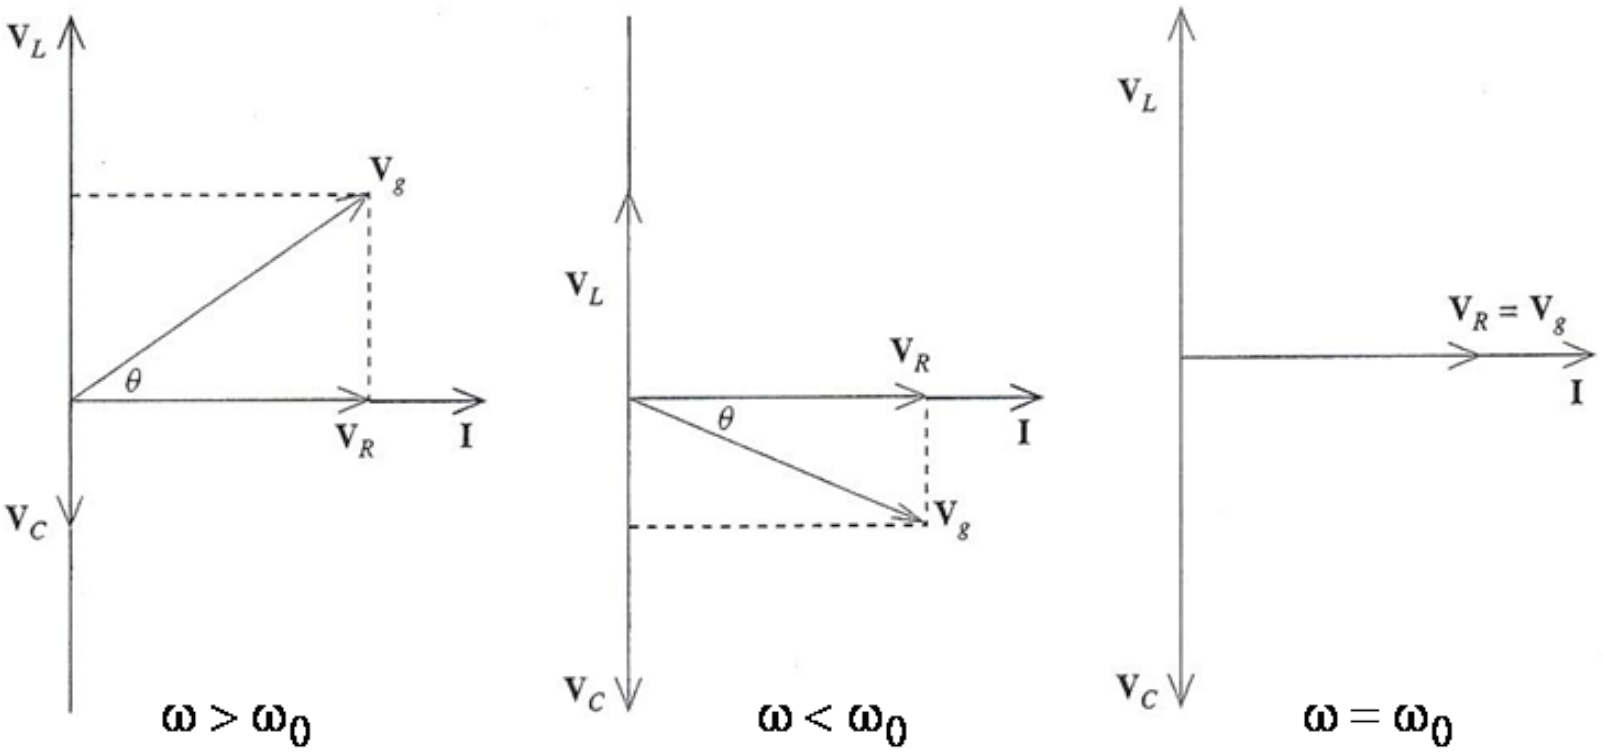
\includegraphics[scale=0.25]{TP3-Exo5.PNG}
\end{center}
}

\Question{0}
{%Q
\textit{La tension $v_C(t)$ peut-elle avoir une amplitude supérieure à celle de la tension d'alimentation?}
}
{%C
Affirmatif, c'est le principe de la résonance.\\
L'amplitude $v_C(t)$ (et $v_L(t)$) peut devenir supérieure à celle de $v_S(t)$. Par contre, $v_R(t)$ ne peut pas dépasser $v_S(t)$.
}

\endinput
